
\section{The Virtual Closed-Loop Prosthesis} \label{sec:vp}

In order to test the usability of the two sensory feedback configurations in a closed-loop control system, a prosthesis which accommodated this was simulated. As no commercial or research prostheses were available in this project, a virtual system resembling prosthetic control was made. Using a virtual prosthesis also had the benefit of providing no sounds that might indicate the position state during evaluation tests.

The aim was to develop a system which could provide control and feedback of two degrees of freedom. In \figref{fig:meth:gridmap} is a depiction of a grid system and a black cursor symbolizing the different possible position states and the current state, respectively, where each square corresponded to a state. Performing supination would make the cursor move to the right into one of two possible states, while performing pronation would make the cursor move left into one of two states. Performing the closed hand movement would make the cursor move downwards into one of four possible hand aperture states and performing open hand would make the cursor move upwards. In total, the prosthesis could achieve a total of 25 different position states, which represented single DoF movements or combinations of two DoFs. However, as the control was sequential it was only possible to move the cursor in a single DoF at a time along an axis. In each of the squares, a unique electrotactile feedback was provided in each of the two feedback configurations, as explained in \secref{sec:feed}.
     

\begin{figure}[H]                 
	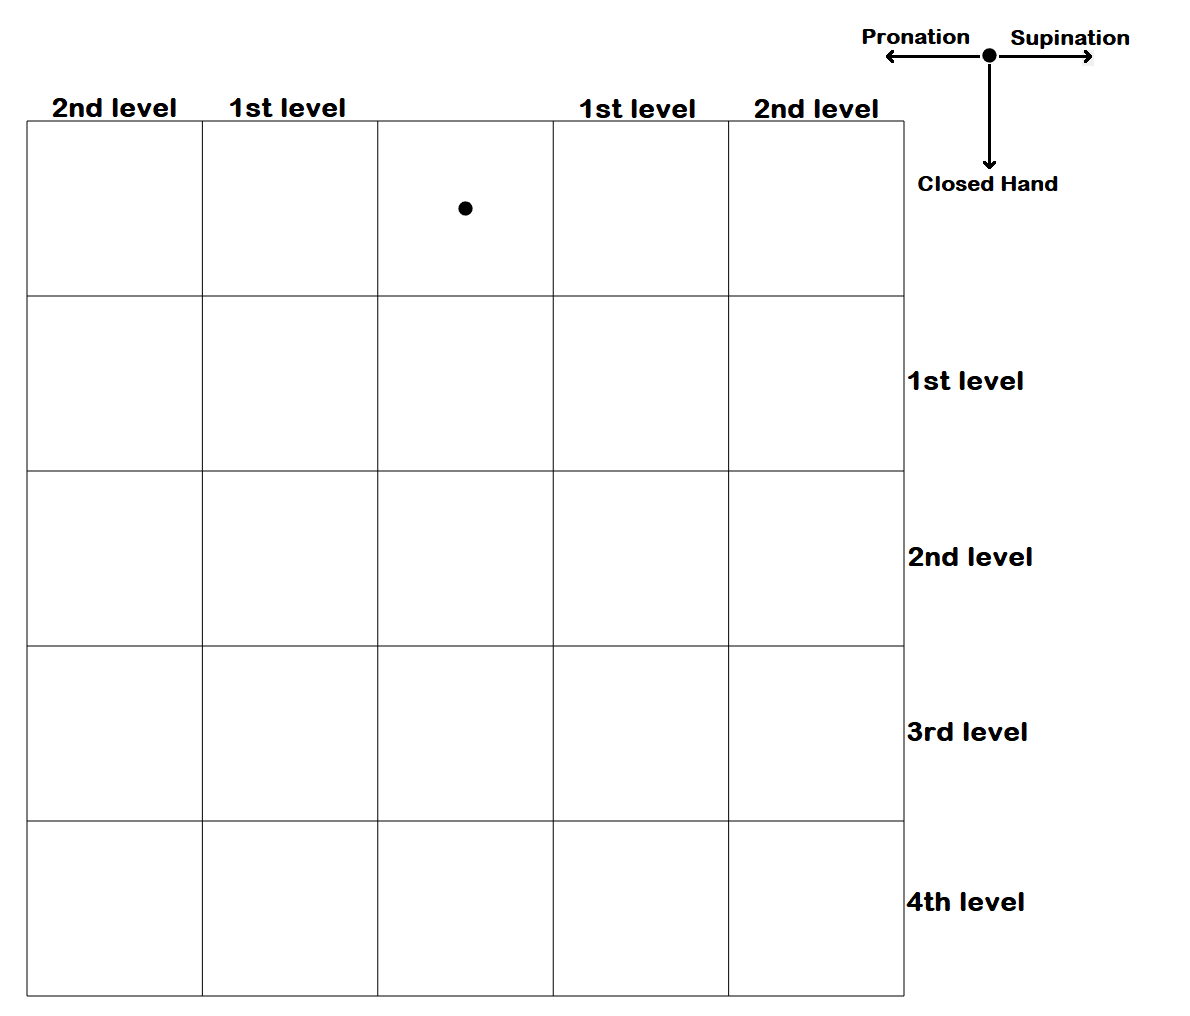
\includegraphics[width=0.9\textwidth]{figures/gridmap2}  
	\caption{Image of the grid map and cursor used in the experiment. Performing supination moved the cursor to the right, pronation moved it to the left and closing the hand moved it downwards. For left handed subjects the rotational movements were reversed. Opening the hand moved the cursor upwards, and was used as a correction movement if needed.}
	\label{fig:meth:gridmap} 
\end{figure}
%hand movements used 

%The Grid 